\documentclass[dvips]{slides}
\usepackage[dvips]{color}
\usepackage{graphics}
\usepackage{dotted}
\usepackage{vdmsl-2e}
\usepackage{mianslides}

\newcommand{\MyM}{\vspace*{-5mm}}
\newcommand{\vpp}{VDM$^{++}$}
\newcommand{\omt}[1]{\resizebox{\textwidth}{!}{\rotatebox{-90}{\includegraphics{#1}}}}


\nolinenumbering
\setindent{outer}{0.0em}

% Toolbox logo
\newbox\ToolboxLogo
\setbox\ToolboxLogo=\hbox{\resizebox{60pt}{!}{\includegraphics{toolbox-logo}}}
\ht\ToolboxLogo=0pt
\dp\ToolboxLogo=0pt
\def\rightup{\mbox{}\kern5.0cm\lower35pt\copy\ToolboxLogo} % rightup is hook into ifadslides.sty
% End Logo


\def\Author{Henrik Voss}
\def\Title{Using OMT and VDM++ for development of a Specification Manager}
\def\Project{Toolbox}
\def\Date{June, 1996}

\renewcommand{\To}{\rightarrow}
\nolinenumbering
\setindent{inner}{.25cm}

\setcounter{page}{0} % We start each chapter on slide page 0
                     % so we don't need to change page numbers 
                     % in succeeding chapter slides. 

\begin{document}

\small
 
\def\titlepage{
   \begin{minipage}{15cm}
     \centerline{Using OMT and \vpp{}}
     \centerline{for development of}
     \centerline{a Specification Manager}
     \centerline{}
     \centerline{\small Henrik Voss}
     \centerline{}
   \end{minipage}
}


\begin{slide}{}
\head{\titlepage}
 \centerline{}
 \centerline{The Institute of Applied}
 \centerline{Computer Science}
 \centerline{}
\end{slide}
 


\begin{slide}{}
\head{Agenda}

\vspace{1cm}
\begin{quote}
\begin{itemize}
\item VDM-SL, \vpp{} and OMT
\item Overview of the VDM-SL Toolbox
\item Architecture and design
\item Use of patterns
\item The approach used
\item Concluding remarks
\end{itemize}
\end{quote}

\end{slide}

\begin{slide}{}
\head{VDM-SL, VDM++ and OMT}

{\bf VDM-SL:}
\small
\begin{itemize}
\item High level type definitions
  \begin{itemize}
  \item Data abstraction
  \item Concentrate on the essential properties
  \end{itemize}
\item Declarative features
  \begin{itemize}
  \item Algorithm abstraction
  \item Enables ``what'' instead of ``how''
  \end{itemize}
\item VDM-SL is being {\bf standardised} by the BSI and the ISO
\end{itemize}

{\bf \vpp{}:}
\small
\begin{itemize}
\item Object Oriented
\item Concurrency
\item Real-Time Features
\end{itemize}

{\bf OMT:}
\small
\begin{itemize}
\item Graphical Notation
\item Methodology
\end{itemize}
\end{slide}



\begin{slide}{}
\head{VDM-SL Toolbox Overview}

\vspace{1cm}
\begin{center}
\resizebox{\textwidth}{!}{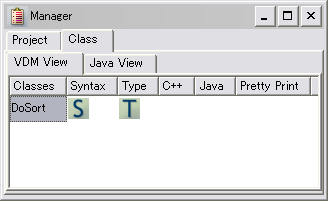
\includegraphics{toolbox.eps}}
\end{center}
\end{slide}


\begin{slide}{}
\head{VDM-SL Toolbox Main Window}

\vspace{1cm}
\begin{center}
\resizebox{\textwidth}{!}{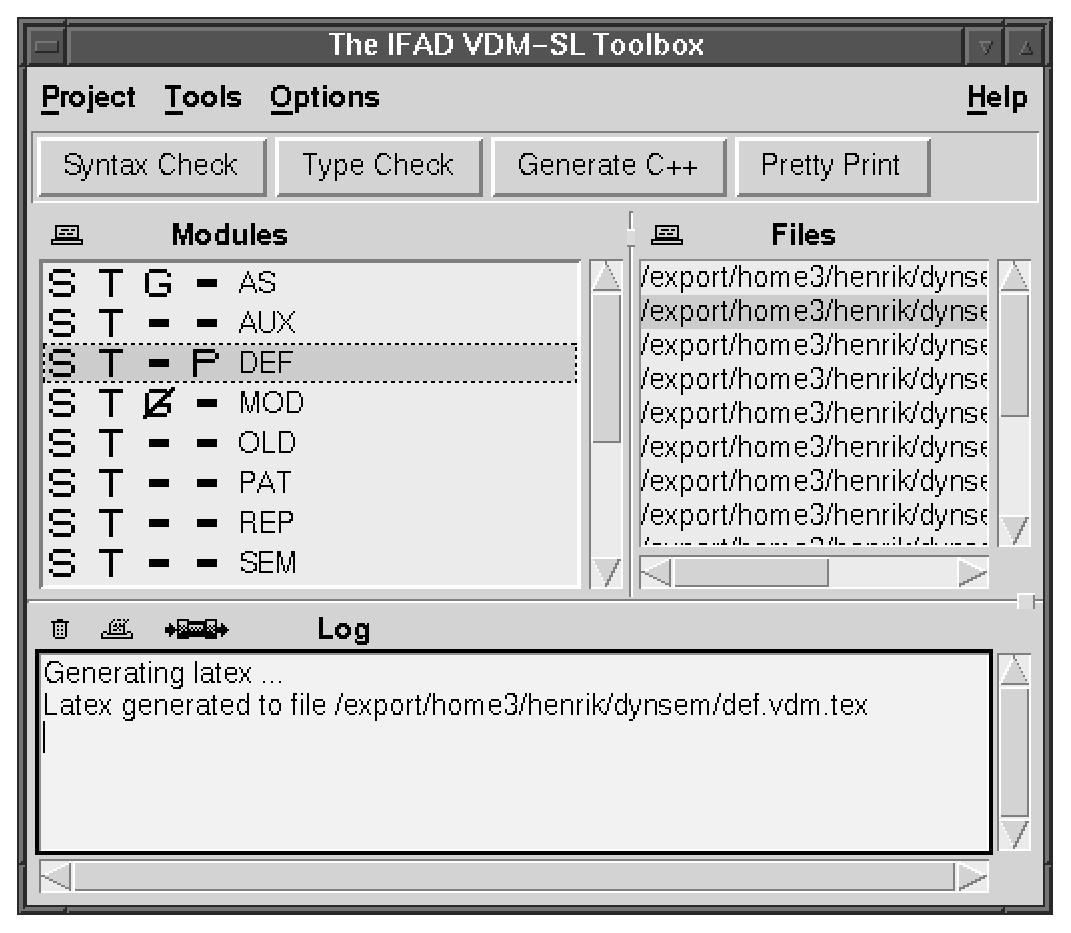
\includegraphics{tbwin.ps}}
\end{center}
\end{slide}



 
\begin{slide}{}
\head{Context Diagram}

\begin{center}
\omt{context.eps}
\end{center}
\end{slide}

\begin{slide}{}
\head{ToolKit -- Mediator View}

{\bf Patterns:} Singleton, Mediator

\begin{center}
\omt{toolkit.eps}
\end{center}
\end{slide}


\begin{slide}{}
\head{Topology}

\begin{center}
\omt{topology.eps}
\end{center}
\end{slide}

\begin{slide}{}
\head{class BaseTools}

{\bf Pattern:} Facade
\begin{center}
\omt{basetools.eps}
\end{center}
\end{slide}


\begin{slide}{}
\head{C++ Interface to BaseTools}

\tiny
\begin{verbatim}
#define VDM_BaseTools 2

#include <math.h>
#include "metaiv.h"
#include "cg.h"
#include "cg_aux.h"
#include "ToolColleague.h"

class vdm_BaseTools : public virtual vdm_ToolColleague {
public:
  virtual void vdm_SetMediator(Class);
  virtual Bool vdm_SyntaxCheck(Sequence);
  virtual Bool vdm_TypeCheck(Sequence);
  virtual Bool vdm_CodeGenerate(Sequence);
  virtual Bool vdm_PrettyPrint(Sequence);
  virtual Tuple vdm_EvalProcess(Record, Record);
  virtual Tuple vdm_ParseExprs(Record);
  virtual Tuple vdm_ParseAndEvalExprs(Record);
  virtual Tuple vdm_ParseAndEvalValue(Record);
  virtual Bool vdm_InitInterpreter();
  virtual Bool vdm_ExecuteCommand(Record);
  virtual Record vdm_EvalFunctions();
  virtual void vdm_InitToolbox();
  virtual void vdm_UpdateToolbox();

  vdm_BaseTools() { class_s.Insert((Int) VDM_BaseTools); }

  virtual ~vdm_BaseTools() {}
};
\end{verbatim}
\end{slide}


\begin{slide}{}
\head{Method: TypeCheck}

\vspace{1cm}
{\bf VDM++:}
\tiny
\begin{verbatim}
TypeCheck (mnm_l: seq1 of ModuleName) value ok: bool
  is not yet specified;
\end{verbatim}

\vspace{1cm}
{\bf Handwritten C++ Code:}
\tiny
\begin{verbatim}
Bool vdm_BaseTools::vdm_TypeCheck (Sequence mnm_l)
{
  bool succ = true;
  
  Errs()->vdm_ClearAll();
  Generic mnm;
  for (int ii = mnm_l.First(mnm);ii;ii = mnm_l.Next(mnm)) {
#ifdef FLM
    Check_lm_periodically();
#endif //FLM
    succ = EvalTypeCheck (mnm) && succ;
  }
  Errs()->vdm_AllDone();
  return Bool (succ);
}
\end{verbatim}
\end{slide}


\begin{slide}{}
\head{class Repository}

\tiny
\begin{verbatim}
instance variables
  cgrepos: @CGRepository;
  unit_m : UnitState;
  file_m : FileState;
  rep    : [FileName];
  session: SessionType;
  storeState: StateType;

  --- rep is the name of the current repository
  --- (nil if no repository is open)

  init objectstate ==
  ( cgrepos := CGRepository!new;
    unit_m  := {|->};
    file_m  := {|->};
    rep := nil;
    session := <NONE>;
    storeState := mk_({|->},{|->})
  )

types
 
  UnitState = map ModuleName to @VDMUnit;

  FileState   = map FileName to FileInfo;
  FileInfo    = ModuleNames * @FileStatus * FileId;
  ModuleNames = set of ModuleName;

  StateType = UnitState * FileState
\end{verbatim}
\end{slide}


\begin{slide}{}
\head{Repository continued}

\tiny
\begin{verbatim}
---
--- Get, add and remove files
--- 

AddFile (file: FileName) ==
  if not file in set dom file_m then
    def fstat : @FileStatus = FileStatus!new in
    ( dcl fileid : nat1 := 1;
      let fileid_s = { id | mk_(-,-,id) in set rng file_m } in
        while fileid in set fileid_s do
          fileid := fileid + 1;
      file_m := file_m munion {file |-> mk_({},fstat,fileid)};
      mediator!CallBack(mk_AddFiles({file})) 
    );

RemoveFile (file: FileName) ==
  if  file in set dom file_m then
    let mk_(unitnm_s,-,-) = file_m (file) in
    ( file_m := {file} <-: file_m;
      unit_m := unitnm_s <-: unit_m;
      mediator!CallBack(mk_RemoveModules(unitnm_s))
    )
\end{verbatim}
\end{slide}



\begin{slide}{}
\head{Error Reporting}

{\bf Pattern:} State

\begin{center}
\omt{error.eps}
\end{center}
\end{slide}


\begin{slide}{}
\head{Error States}

\begin{center}
\omt{errorstate.eps}
\end{center}
\end{slide}




\begin{slide}{}
\head{The Approach Used}

\vspace{1cm}
\begin{itemize}
\item Handwrite OMT class and event trace diagrams.
\item Use patterns as inspiration.
\item Write \vpp{} classes and methods.
\item Generate C++ code.
\item Integrate C++ code with existing code.
\item Run integration tests.
\item Generate OMT object Model.
\item Use \vpp{} and OMT as documentation in the maintenance phase
\end{itemize}
\end{slide}


\begin{slide}{}
\head{Concluding Remarks}

\vspace{1cm}
{\bf Advantages:}
\begin{itemize}
\item No implementation details in the design.
\item Consistency between documentation and implementation.
\item \vpp{}: operations early in the design.
\item OMT and \vpp{} are good communication mediums in the development
  team.
\item \vpp{} provides an unambiguous design model and pseudo code language.
\item \vpp{} code generation enables early prototyping.
\end{itemize}

{\bf Drawbacks:}
\begin{itemize}
\item Generated code less efficient than handwritten code.
\item Conversion functions needed.
\end{itemize}

\end{slide}



\end{document}



